% Chapter 2

\chapter{Background Information and Theory} % Main chapter title
\label{Chapter2} % For referencing the chapter elsewhere, use \ref{Chapter2} 


%----------------------------------------------------------------------------------------

This chapter gives necessary background information for the topics covered in this thesis. 

\section{Motivation for Using Machine Learning to Improve the Indoor Tracking System}

The Indoor Tracking System, hereafter referred to as ITS, (\cite{indoor_tracking_system_smartphones, tracking_system_fuse, fine_grained, sensor_fusion}) can continuously predict the user's location based on the location of the user a short time ago and the orientation and movement of the device. Basically, it suggests a collection of possible points the user could be at. It can predict the user's location with an accuracy of 1.7 meters.

The aim of the indoor localization system presented in this thesis (hereafter referred to as Indoloc) is to improve the accuracy of the ITS using ML. We hope that this can be done by excluding all the possible locations of the user of one room if the Indoloc predicts the other and by using landmarks. A landmark is defined as a small area within a room. Thus, when a landmark is recognized by Indoloc, the ITS can then tell with high confidence that it is located in a certain very small area. This makes the ITS more precise. (\cite{continuous_indoor_positioning, indoor_positioning_method})

Figure \ref{fig:LandmarksChapter2} shows how Indoloc can improve the ITS. The red points symbolize the collection of possible locations the user could be at, suggested by the ITS. The five boxes represent the landmarks. These landmarks are small imagined areas inside a room. Indoloc predicts the landmark "top left" with the green background. As a consequence, the ITS can exclude the points which are far away, namely the ones crossed out.


\begin{figure}[H]
\centering
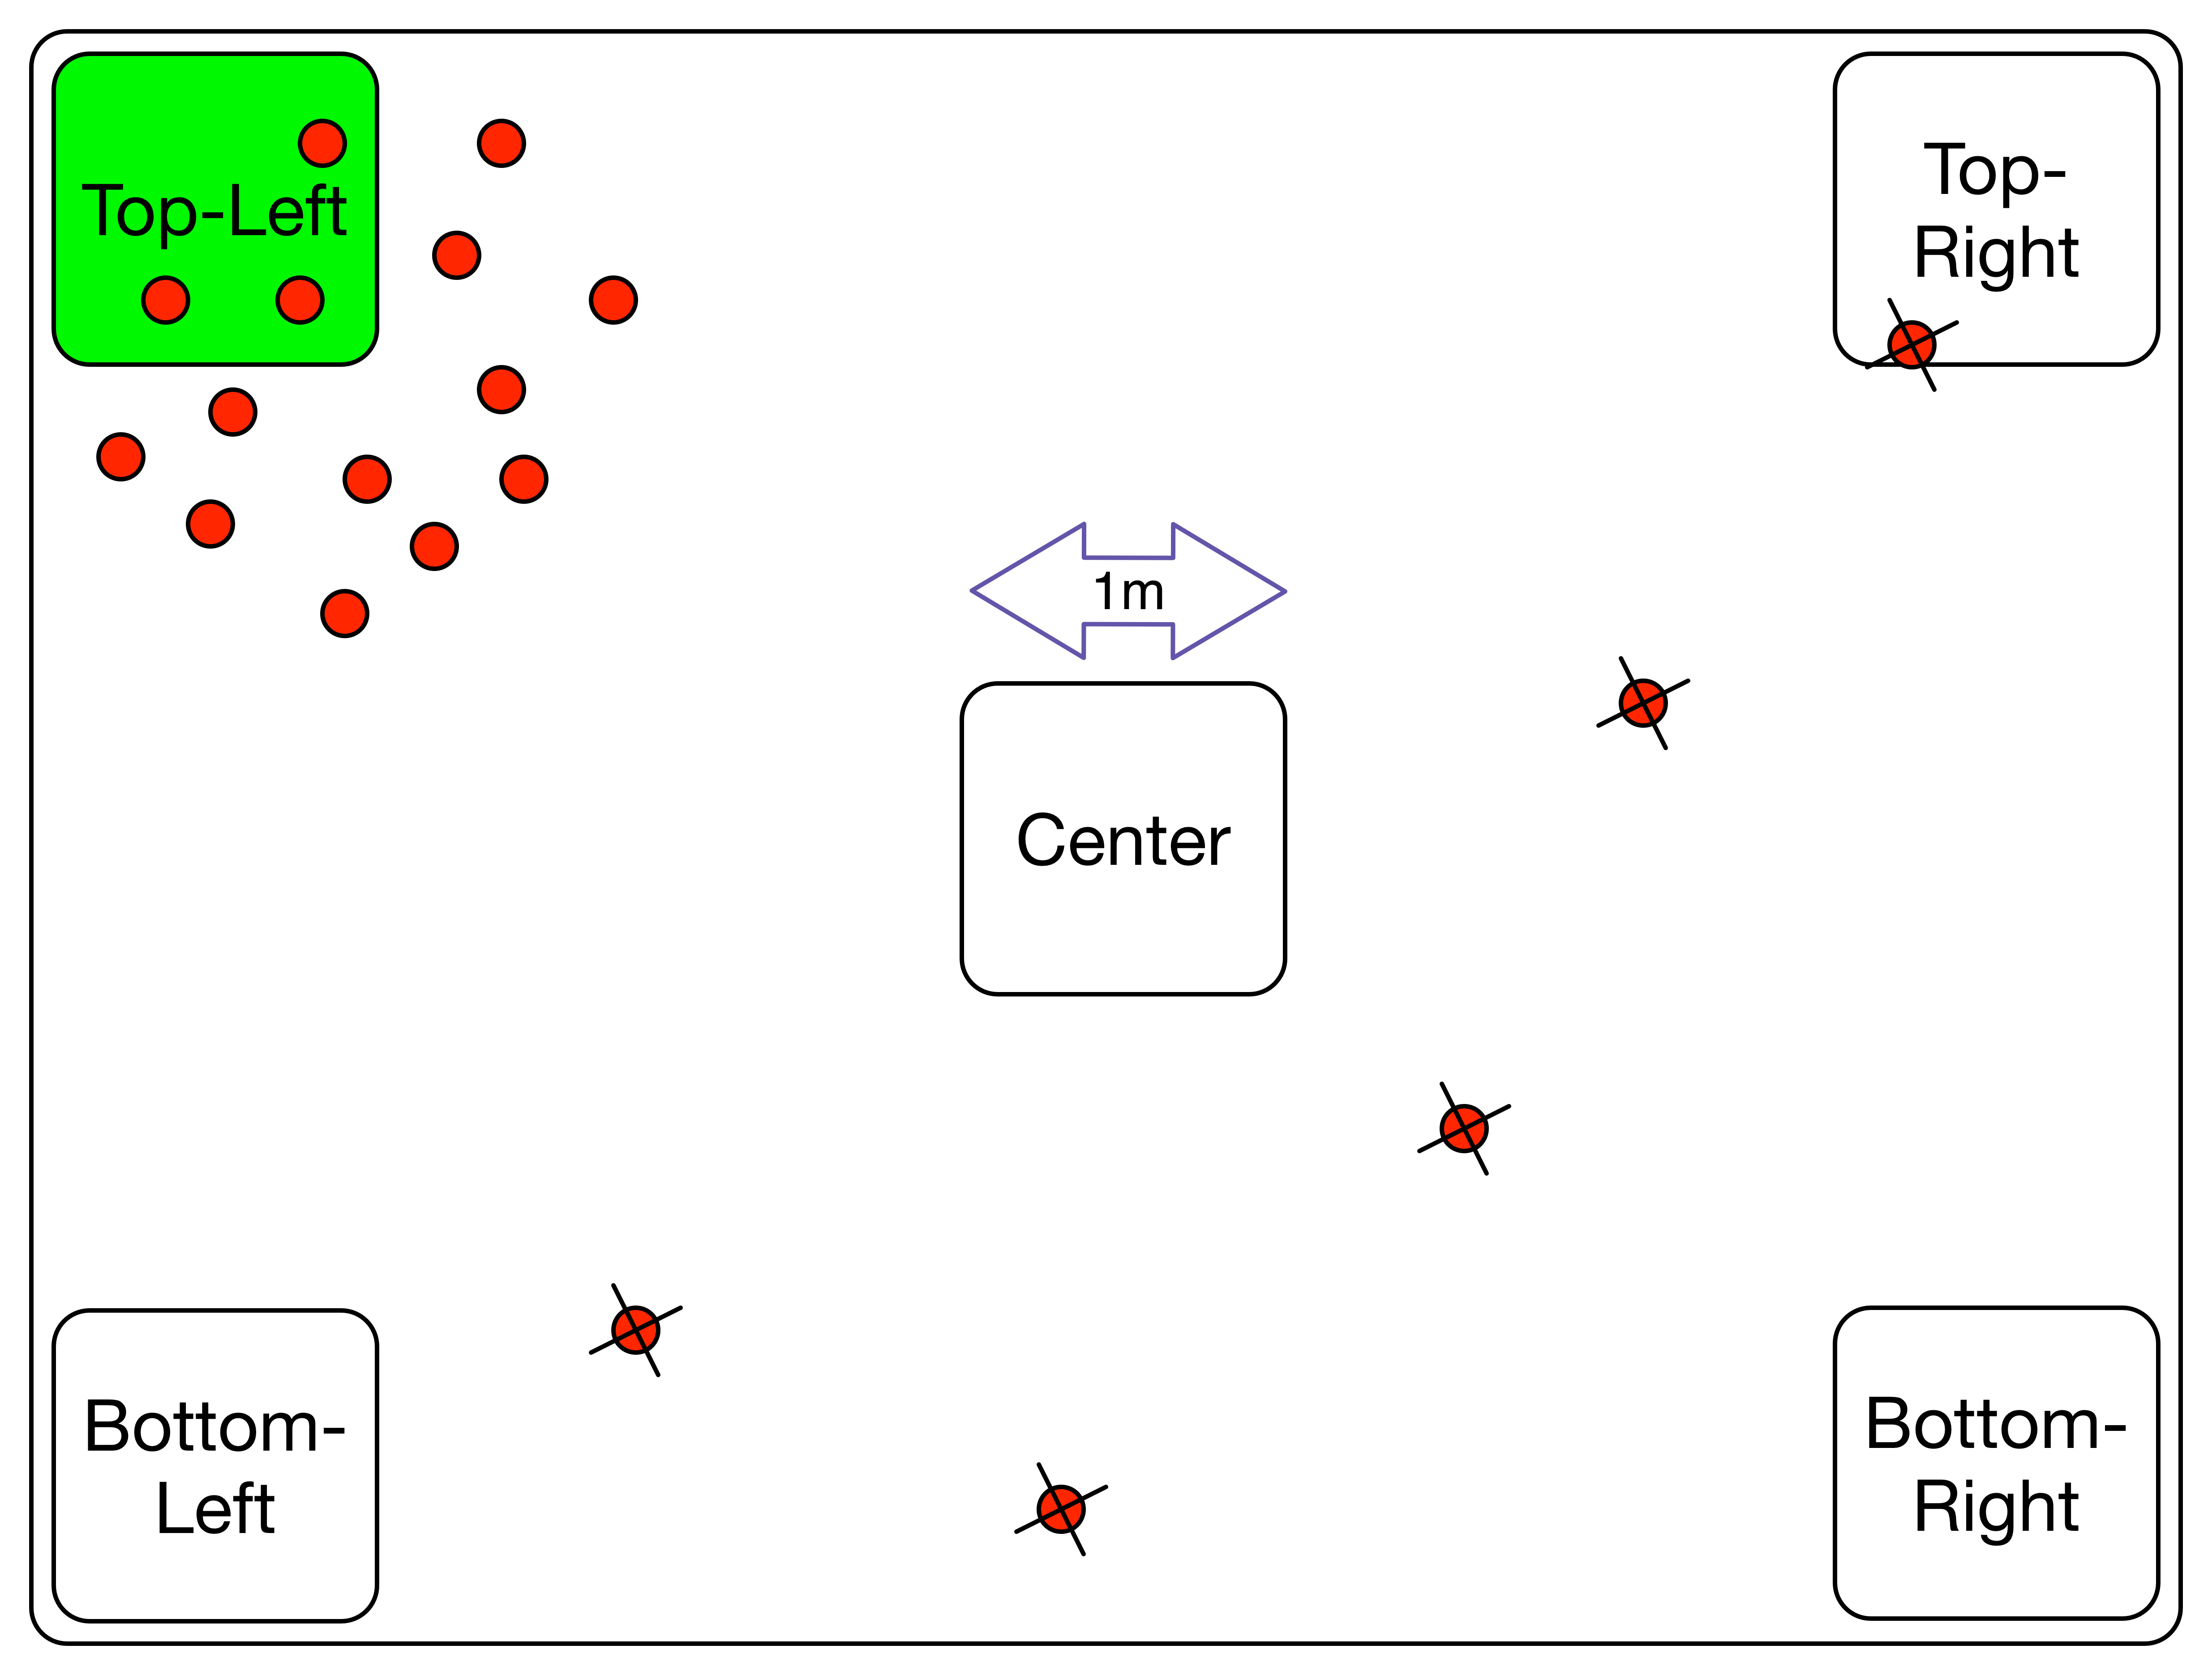
\includegraphics[width=100mm]{Figures/Landmarks.jpg}
\decoRule
\caption[Landmarks]{Five landmarks and the collection of red points predicted by the ITS.}
\label{fig:LandmarksChapter2}
\end{figure}

%----------------------------------------------------------------------------------------

\section{Reasons for Using Machine Learning}
Machine Learning is very suitable for analyzing big amounts of data. The supervised learning methods that are used in this work read the given training data and then build a model of it, which tries to distinguish the given classes. This model can then be applied to the data points collected by the user during the experiment and, in this way, it can predict the class (room or landmark respectively) of the user. By using Machine Learning methods we can take advantage of the modern smart phone's ability to collect huge amounts of data about what is happening around it.


%----------------------------------------------------------------------------------------


\section{Machine Learning Workflow}
\label{sec:MLWorkflow}

In this section we are giving a short introduction about the workflow we used to achieve the best accuracy possible for the tested datasets. We used an article about a typical machine learning workflow (\cite{ml_workflow}) as a guideline for our workflow.
%and the menu of the Weka explorer in the graphical user interface of the Weka application seen in Figure \ref{fig:WekaExplorer} 

% \begin{figure}[H]
% \centering
% 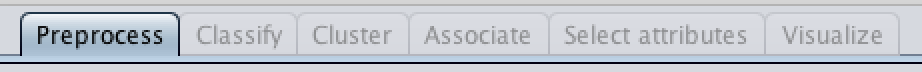
\includegraphics[width=100mm]{Figures/WekaExplorer.jpg}
% \decoRule
% \caption[Weka Explorer]{The menu of the Weka explorer in the graphical user interface of the Weka application.}
% \label{fig:WekaExplorer}
% \end{figure}


\begin{enumerate}
\item \textbf{Data Preprocessing} \\
First, the data has to be cleaned. Redundant or insensible information has to be deleted. 
\item \textbf{Attribute Selection} \\
Second, the right attributes have to be selected. Some attributes may not contribute any useful information to the model and can therefore be discarded. Specifically for this thesis it is discussed in Section \ref{sec:AttributeSelection} and \ref{sec:AttributeExclusion}.
\item \textbf{Feature Engineering} \\
In this part of the workflow, we try to create new features, for instance in Section \ref{sec:MeanAndVariances}, or modify existing features to improve the accuracy (Section \ref{sec:Rounding}).
\item \textbf{Find Base Learners} \\
In this section, we find the best base ML method.
\item \textbf{Find Meta Learners} \\
In this step, we improve the performance using meta learners. A meta learner is defined as a combination of one or several different base learners (conventional ML algorithm). This is described in more detail in Section \ref{sec:Ensemble}.
\item \textbf{Hyper-Parameter search} \\
Finally, we use methods like autoweka, gridsearch, multisearch or trial-and-error to tweak the parameters of the chosen ML methods in order to further improve the accuracy (Section \ref{sec:HyperParameterSearch}).
\end{enumerate}

This workflow is an iterative process. In order to achieve the best results it may have to be repeated several times.


%----------------------------------------------------------------------------------------

\section{Chosen Machine Learning Algorithms}
As Weka provides a very big amount of efficiently implemented machine learning algorithms we could test lots of them without spending efforts of implementing them from scratch. An overview can be found on \url{http://wiki.pentaho.com/display/DATAMINING/Classifiers}. The following list includes the algorithms that have been implied in this thesis. Detailed information about the algorithms can be found in the method \texttt{addClassifiers()} in the class \url{https://github.com/JoelNiklaus/IndoLoc/blob/master/app/src/test/java/ch/joelniklaus/indoloc/AbstractTest.java}.

\begin{itemize}
   \item Bayes
   \begin{itemize}
     \item NaiveBayes (see \cite{John1995})
   \end{itemize}
   
   \item Functions
   \begin{itemize}
     \item LibSVM (Library for Support Vector Machines, see \cite{libsvm})
     \item Logistic (see \cite{leCessie1992})
     \item MultilayerPerceptron (Neural Network)
     \item SMO (Sequential Minimal Optimisation) (see \cite{Platt1998, Keerthi2001, Hastie1998})
   \end{itemize}
   
   \item Trees
   \begin{itemize}
     \item J48 (see \cite{Quinlan1993})
     \item RandomForest (see \cite{Breiman2001})
   \end{itemize}
   
   \item Lazy (Instance Based)
   \begin{itemize}
     \item IBk (Implementation of the K-Nearest-Neighbour Algorithm, see \cite{Aha1991})
     \item KStar (see \cite{Cleary1995})
     \item LWL (Locally Weighted Learning, see \cite{Frank2003, Atkeson1996})
   \end{itemize}
   
   \item Meta
   \begin{itemize}
     \item AdaBoostM1 (Adaptive Boosting, see \cite{Freund1996})
     \item Bagging (see \cite{Breiman1996})
     \item Dagging (see \cite{Ting1997})
     \item Decorate (see \cite{Melville2003, Melville2004})
     \item Grading (see \cite{Seewald2001})
     \item LogitBoost (see \cite{Friedman1998})
     \item RandomSubSpace (see \cite{Ho1998})
     \item Stacking (see \cite{Wolpert1992})
     \item Vote (see \cite{Kuncheva2004, Kittler1998})
   \end{itemize}
\end{itemize}

Because an explanation of all the tested algorithms would go beyond the constraints of this thesis we are giving the following recommendations for the interested reader: A good website to get an overview on \url{http://machinelearningmastery.com/a-tour-of-machine-learning-algorithms/} and a good article for more details on \url{http://alex.smola.org/drafts/thebook.pdf}.


%----------------------------------------------------------------------------------------

\section{Features}
\label{sec:Features}
In a Machine Learning project the attributes of the classes are denoted as features. Each feature is describing an aspect of the classes. In our case features are our measurements, for instance an RSS value. For the ML project to deliver a good prediction accuracy it is very important to select the right attributes/features and to also modify certain features or even create new features out of existing features. This is part of the ML workflow described in Section \ref{sec:MLWorkflow}.

In the following sections both the features used in the system and the ones taken into consideration, but then found to be useless, are introduced. Each feature corresponds to one column in the dataset and would be referred to as an attribute in Weka.

\subsection{Features used in the experiments}

In the following sections, the features which are actually used in the running system are presented.


\subsubsection{RSS}
\label{sec:RSS}
The RSS values provide the core data as they contribute the most to the performance of the ML methods. The smart phone scans the surrounding access points, obtains and registers the RSS values of each access point. These values depend on the distance to the access point as well as on the existence of obstacles, such as walls or furniture, between the access point and the device. Normally the RSS values in our datasets were between -20 and -90.

\subsubsection{Magnetic Field}
\label{sec:MagneticField}

%http://www.eecs.yorku.ca/course_archive/2014-15/W/4443/DemoPrograms/demoflat/DemoFlatActivity.html

\begin{figure}[H]
\centering
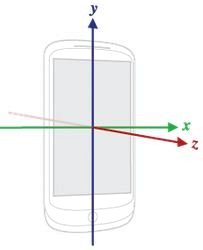
\includegraphics[width=100mm]{Figures/Device.jpg}
\decoRule
\caption[Device]{The values in the device's coordinate system.}
\label{fig:Device}
\end{figure}

\begin{figure}[H]
\centering
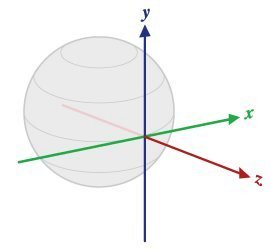
\includegraphics[width=100mm]{Figures/Earth.jpg}
\decoRule
\caption[Earth]{The values in the earth's coordinate system.}
\label{fig:Earth}
\end{figure}

The device's sensors measure the magnetic field in the device's coordinate system. As the user walks around, the orientation of the device may change all the time. We would therefore have to collect all possible values from every orientation in every point for the training phase. This would result in a huge amount of data and the training performance would be extremely inaccurate. 


In addition to the raw magnetic field values we can also derive data from the accelerometer measuring gravity in the device's coordinate system. By using the Android built in function \texttt{SensorManager.getRotationMatrix()} and providing the magnetic field and gravity values, we can get the rotation matrix \texttt{R} and the inclination matrix \texttt{I}.
Using these two matrices, we have two methods making use of the raw data (coded in \url{https://github.com/JoelNiklaus/IndoLoc/blob/master/app/src/main/java/ch/joelniklaus/indoloc/models/SensorData.java}):



\paragraph{Magnetic Processed}

With the help of \texttt{R} we then can do a change of the basis from the device's to the earth's coordinate system to get the processed magnetic values \texttt{mp}. (see \ref{magneticProcessedEq})

\begin{equation} \label{magneticProcessedEq}
\begin{pmatrix}
0 \\
mp \\
mp
\end{pmatrix} 
 = R * m
\end{equation}

Now we have got the magnetic field data at a specific point in the earth's coordinate system. The x value is in East-West Direction, the y value is in North-South Direction and the z value is perpendicular to the center of the earth. As the magnetic field of the earth only goes from one pole to the other the x value is always 0 and is therefore not used as a feature.


\paragraph{Gravity Magnitude and Geomagnetic Magintude}
In order to obtain the gravity magnitude \texttt{grm} (in z direction) we multiply the gravity vector \texttt{g} with \texttt{R}. (see \ref{gravityMagnitudeEq})


\begin{equation} \label{gravityMagnitudeEq}
\begin{pmatrix}
0 \\
0 \\
grm
\end{pmatrix} 
 = R * 
\begin{pmatrix}
g_1 \\
g_2 \\
g_3
\end{pmatrix}
\end{equation}


To obtain the geomagnetic magnitude \texttt{gem} (in y direction) we multiply the magnetic vector \texttt{m} with $I*R$. (see \ref{geomagneticMagnitudeEq})

\begin{equation} \label{geomagneticMagnitudeEq}
\begin{pmatrix}
0 \\
gem \\
0
\end{pmatrix} 
 = I * R * 
\begin{pmatrix}
m_1 \\
m_2 \\
m_3
\end{pmatrix}
\end{equation}

\paragraph{Additional information}
In order to reduce extreme variations which might disturb the ML algorithms, we apply a low-pass-filter to the newly collected data. For the alpha value we chose 0.75. So the last value has a weight of 0.75 and the newly collected value a weight of 0.25.
The accuracy of the magnetic field sensor in the devices we tested is 0.15 \textmu T. But still the data the sensor outputs contains many more decimal places. In order to exclude the noise, we round the values to 1 \textmu T. 
The values obtained by measuring the magnetic field provide an improvement to the overall accuracy.



\subsubsection{Light}
We also thought about including data collected from the light sensor because, for instance, a room facing a window will clearly be brighter than one surrounded by walls only. As can be seen in Section \ref{AdditionalFeatures} this does improve the prediction accuracy, however, these assumptions are not stable over time. In the night, there may be no difference concerning light at all between the two previously mentioned rooms. Or if there is a cloudy day the overall light strength would probably be much less as compared to that on a sunny day. Thus, it might be appropriate to work with light differences to a representative data point. This data point would have to be chosen carefully and would have to be recorded first. 

We include this suggestion here because it improves the result but it still has to be tested if it is worth integrating it into a system in a productive environment.


\subsection{Non-useful features}
In the following sections the features which have been taken into account but have been judged as not helpful are presented. These features are therefore not included into the running system, as they would only produce additional overhead and slow down the generation and evaluation of the ML models.

\subsubsection{Ambient temperature}
At first we thought about including the ambient temperature as another feature because there may be characteristic small temperature differences between rooms which could help in making predictions.

However, we estimate this feature to be rather unpredictable. For instance when someone turned the heating up in one specific room, the temperature would change drastically. As a consequence, we would suddenly receive incredibly conflicting values. Or imagine someone opens the window on a very cold day. Even without any human interference, different seasons or poor isolation of walls or windows could have an influence on temperatures in the same room.
Apart from that, there are still lots of devices which do not yet have any temperature sensors.

\subsubsection{Relative Humidity}
Another idea would have been to include relative humidity. In comparing a bathroom and an office, for instance, it would be a fair assumption that the relative humidity would be higher in the former than the latter.
But, as with the ambient temperature, we think that it is too volatile overall. An open window on a rainy day or even just a hot steaming tea can change the humidity landscape of a room. And here as well, there are not many devices which already have a relative humidity sensor built in.


\subsubsection{Pressure}
Relative pressure differences are utilized in the ITS to distinguish between different floors of a building. But this work is only part of the ITS and only has to provide predictions on the same floor. Therefore, it does not make sense to include it in this system. Furthermore, the Motorola test device was not even equipped with a pressure sensor.

\subsubsection{Mean and Variances of RSS}
\label{sec:MeanAndVariances}
One idea was to include the mean and the variances of the RSS values. But as experiments have been able to show, this does not improve the overall accuracy. This is probably the case because it does not add additional information to the ML algorithms but just alters and adds pre-existing ones.


\subsubsection{GPS}
An idea is to include the latitude and longitude gained from the GPS to help prediction close to the windows. But as our tests in Section \ref{AdditionalFeatures} have shown the accuracy is decreased if it is included.


%----------------------------------------------------------------------------------------

\section{Weka}
Weka, standing for Waikato Environment for Knowledge Analysis, is an open source machine learning library programmed in Java developed by the University of Waikato, New Zealand, and can be found on \url{http://www.cs.waikato.ac.nz/~ml/weka/}.

Two reduced versions for Android \footnote{rjmarsan: \url{https://github.com/rjmarsan/Weka-for-Android}} \footnote{Shookit: \url{https://github.com/Shookit/android-ml-weka}} have been considered and the first version (from the developer with user name rjmarsan) has been chosen. It uses Weka 3.7.3 and mainly does not include the GUI (Graphical User Interface) parts of the system which are not used in this application.

\subsection{Advantages}
The main reason why we chose the library Weka, is the huge amount of efficiently implemented ML algorithms it provides. It offers a wide range of both supervised and unsupervised learning algorithms. Furthermore, in addition to the Java interface there is both a command line interface and a graphical user interface available.

\subsection{Disadvantages}
Although the introduction documentation \footnote{Programmatic Use: \url{https://weka.wikispaces.com/Programmatic+Use}} \footnote{Weka in Java Code: \url{https://weka.wikispaces.com/Use+WEKA+in+your+Java+code}} provides you with some information to get started, the Javadoc \footnote{Javadoc: \url{http://weka.sourceforge.net/doc.stable/}} is not of much use. It only provides one very small sentence to most of the methods (functions). This sentence mostly does not add any additional details to the information from the method's name. 

The Javadoc for the classes is slightly better though, providing some explanation how to use it. The design of the methods is very close to the use of the command line. So usually a string array of cryptic options has to be provided in order to configure the classifier. Sometimes it can be done using setter methods, but if so it is poorly documented what exactly is altered by setting a certain value.

There is a mailing list \footnote{Mailing List: \url{https://list.waikato.ac.nz/mailman/listinfo/wekalist}} and a forum on Pentaho \footnote{Pentaho Forum: \url{http://wiki.pentaho.com/display/DATAMINING/Pentaho+Data+Mining+Community+Documentation}} where questions concerning Weka can be asked. But unfortunately the active community does not seem to be very large. For my problems at least, we had great difficulties finding answers through these two channels.


%----------------------------------------------------------------------------------------


\section{Android App}

\subsection{Implementation}
If the reader is interested in knowing how to implement an Android app we can recommend the following web resources: Android Developers on \url{https://developer.android.com/index.html} and Android Studio on
\url{https://developer.android.com/studio/index.html}.



\subsection{Reasons for Choosing the Android System}
The most important reason which lead to the choice of Android as a (first) platform of the app was the ITS which is being implemented in Android. On top of that, Weka offers a Java interface which makes it very easy to integrate into an Android app.

\subsection{Tested Mobile Phones}

First, we tested the Android app on the Emulator in Android Studio. This was fine for examining how the user interface behaved but after we added the WiFi, Sensor and GPS collection, we had to test it on real phones. We used the following two Android phones:
Nexus 4 (LG, Android Version 5.0, API, Level 22, Accurate Specifications on  \url{https://en.wikipedia.org/wiki/Nexus_4}) and Moto X Style (Motorola, Android Version 6.0, API Level 24, Accurate Specifications on  \url{https://www.digitec.ch/en/s1/product/motorola-moto-x-style-570-32gb-21mp-black-mobile-phones-5339851}).
%----------------------------------------------------------------------------------------




